\subsection{Quel paysage des réseaux explore-t-on ?}
\label{sec:paysage}

% Brouillon rédigé par Claude (2026-10-04), à reprendre dans la voix de Quentin. Il suit les puces
% de Quentin dans leur ordre ; les captures sont à faire (fiches P0 à P5 de plan_figures.md).
La pluripotence, telle que l'introduction la définit, peut prendre plusieurs formes dans le formalisme des SBN, et nous les présentons ici de celle que ce travail explore le plus à celles qu'il laisse de côté.

La première passe par les nœuds de contrôle.
Un nœud $c$ est un nœud de contrôle quand il garde toujours sa valeur, $f_c(\mathbf{x}) = x_c$ pour tout état $\mathbf{x}$, si bien que les deux faces $x_c = 0$ et $x_c = 1$ de l'hypercube sont invariantes et portent chacune une sous-dynamique de dimension $n-1$, que le réseau « simule » selon la valeur de $c$ (\Cref{fig:reseau-pluripotent-3d}).
% Fiche P1 supprimée (Quentin, 2026-10-04) : doublon de la figure X2 des Motivations.
Le rapport de Danwen~\cite{wu2024} montre que cette propriété se lit directement sur les poids, puisque $c$ est un nœud de contrôle si et seulement si
\begin{equation}
\sum_{i \neq c} \max(0, w_{i,c}) \le 0
\qquad \text{et} \qquad
w_{c,c} + \sum_{i \neq c} \min(0, w_{i,c}) > 0 ,
\end{equation}
c'est-à-dire si aucun autre nœud ne peut l'allumer (ses arcs entrants sont inhibiteurs ou absents) ni l'éteindre (sa boucle l'emporte sur toutes les inhibitions réunies).
% src : wu2024, définitions 1.7 à 1.10 et proposition 4.1 (closure constraints, écrites avec |w_ic|,
% équivalentes puisque la première condition impose w_ic <= 0) ; PTBN_undercontrol.lp (pos_w, neg_w)
Chaque face peut à son tour avoir un nœud de contrôle parmi les nœuds restants, et ainsi de suite, de sorte qu'une dynamique se décompose selon un arbre dont chaque nœud interne est une coupe selon un nœud de contrôle et chaque feuille un sous-cube invariant qui n'est plus coupé.
Le vecteur de décomposition $\langle v_n, \dots, v_0 \rangle$ compte les feuilles de chaque dimension, $v_k$ étant le nombre de feuilles de dimension $k$, du vecteur trivial $\langle 1, 0, \dots, 0 \rangle$, qui ne coupe rien, à $\langle 0, \dots, 0, 2^n \rangle$, où tous les états sont des points fixes.
Ces décompositions sont complètes, au sens où leurs feuilles recouvrent tout l'hypercube, et ce sont elles qu'énumèrent nos programmes (\Cref{sec:correction}).


Reste à savoir ce que sont ces sous-dynamiques.
Sur la face $x_c = 0$, le nœud $c$ éteint ne contribue à rien et la sous-dynamique est celle du réseau restreint aux autres nœuds, donc celle d'un SBN, mais sur la face $x_c = 1$, chaque nœud $j$ reçoit en permanence le poids $w_{c,j}$, qui joue le rôle d'un seuil, si bien que la sous-dynamique est celle d'un réseau de fonctions à seuil quelconques (TBN, pour \emph{Threshold Boolean Network}), qui n'est pas forcément un SBN.
Nous reprenons l'appellation de la HDR de Nicolas~\cite{glade2022}, où une fonction booléenne à seuil (TBF) vaut 1 quand la somme pondérée de ses entrées dépasse strictement un seuil propre au nœud, et où toute TBF se simule justement par une SBF recevant d'un nœud toujours allumé un arc de poids opposé au seuil, ce que fait ici le nœud de contrôle.
% src : glade2022, section 8.3.3.2.c, p. 161-162 (équation 1, figure 8.30 : nœud auto-activé initialisé à 1,
% arc de poids -theta) ; même construction dans segretain2023, introduction, figure 3
Nous appelons donc PTBN un réseau pluripotent dont les sous-dynamiques sont des TBN, et PSBN un réseau dont chaque sous-dynamique est celle d'un SBN de dimension inférieure, ce qui demande l'existence, pour la face $x_c = 1$, de poids $w'_{i,j}$ tels que
\begin{equation}
\sum_{i \neq c} w_{i,j}\, x_i + w_{c,j} > 0
\iff
\sum_{i \neq c} w'_{i,j}\, x_i > 0
\qquad \forall\, j \neq c,\ \forall\, \mathbf{x} \text{ tel que } x_c = 1 ,
\end{equation}
et de même à chaque niveau de l'arbre, avec la somme des poids venant des nœuds de contrôle allumés.
% src : PSBN_undercontrol.lp (offset et poids w(I,J,context) des sous-réseaux) ; wu2024, section 5
Un SBN envoyant toujours sur lui-même l'état où tous ses nœuds sont éteints (aucune somme n'y est positive), il faut en particulier $w_{c,j} \le 0$ pour tout $j \neq c$~\cite{wu2024}, et c'est ce qui manque à la dynamique de la \Cref{fig:ptbn-3d}, dont la face $x_3 = 1$ envoie l'état 100 sur 101.
% src : wu2024, proposition 5.1 (« in particular w_nj <= 0 ») ; plan_figures.md (vérification de sbn71)
L'écart entre les deux notions est grand, puisqu'en dimension 3, 2\,977 dynamiques ont au moins un nœud de contrôle, mais 658 seulement se décomposent en SBN.
Ces dynamiques se comptent sans être énumérées, car les colonnes de $W$ étant indépendantes, il suffit de savoir, pour chaque SBF, si sa restriction à une face $x_c = 1$ est encore une SBF, puis de compter les $n$-uplets de SBF qui ont au moins un nœud de contrôle dont toutes les autres colonnes passent ce test.
La pluripotence devient ainsi très vite rare (\Cref{tab:echelles}), les dynamiques décomposables en SBN ne représentant que 2~\% des dynamiques en dimension 3, 0,06~\% en dimension 4 et 0,0003~\% en dimension 5.
% src : comptage par colonnes du 2026-10-05 (5 et 658 en d = 2 et 3, comme les CSV de JPP)
% src : passe unifiée ae10d77 (fiches C4 et P2 : 658 dynamiques non triviales en PSBN, 2 319 non
% triviales en PTBN seulement) ; 2 977 = 32^3 - 31^3

% Fiche P2 : figure existante (1er juillet), vérifiée le 2026-10-04 : le réseau réalise exactement
% l'hypercube, et la dynamique n'a que le vecteur trivial en PSBN. Elle illustrait jusqu'ici les
% Motivations, où la fiche X2 la remplace.
\begin{figure}[H]
    \centering
    \begin{subfigure}{0.48\linewidth}
        \centering
        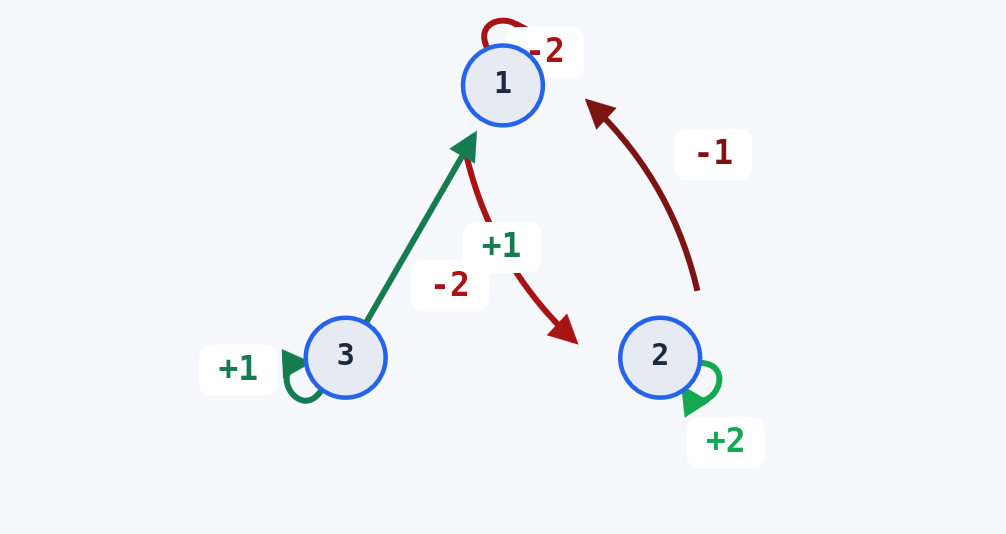
\includegraphics[width=\linewidth]{figures/3d__0_2_0_0__PTBN_undercontrol_taggedtree_sbn71_reseau.png}
        \caption{La structure.}
    \end{subfigure}
    \hfill
    \begin{subfigure}{0.48\linewidth}
        \centering
        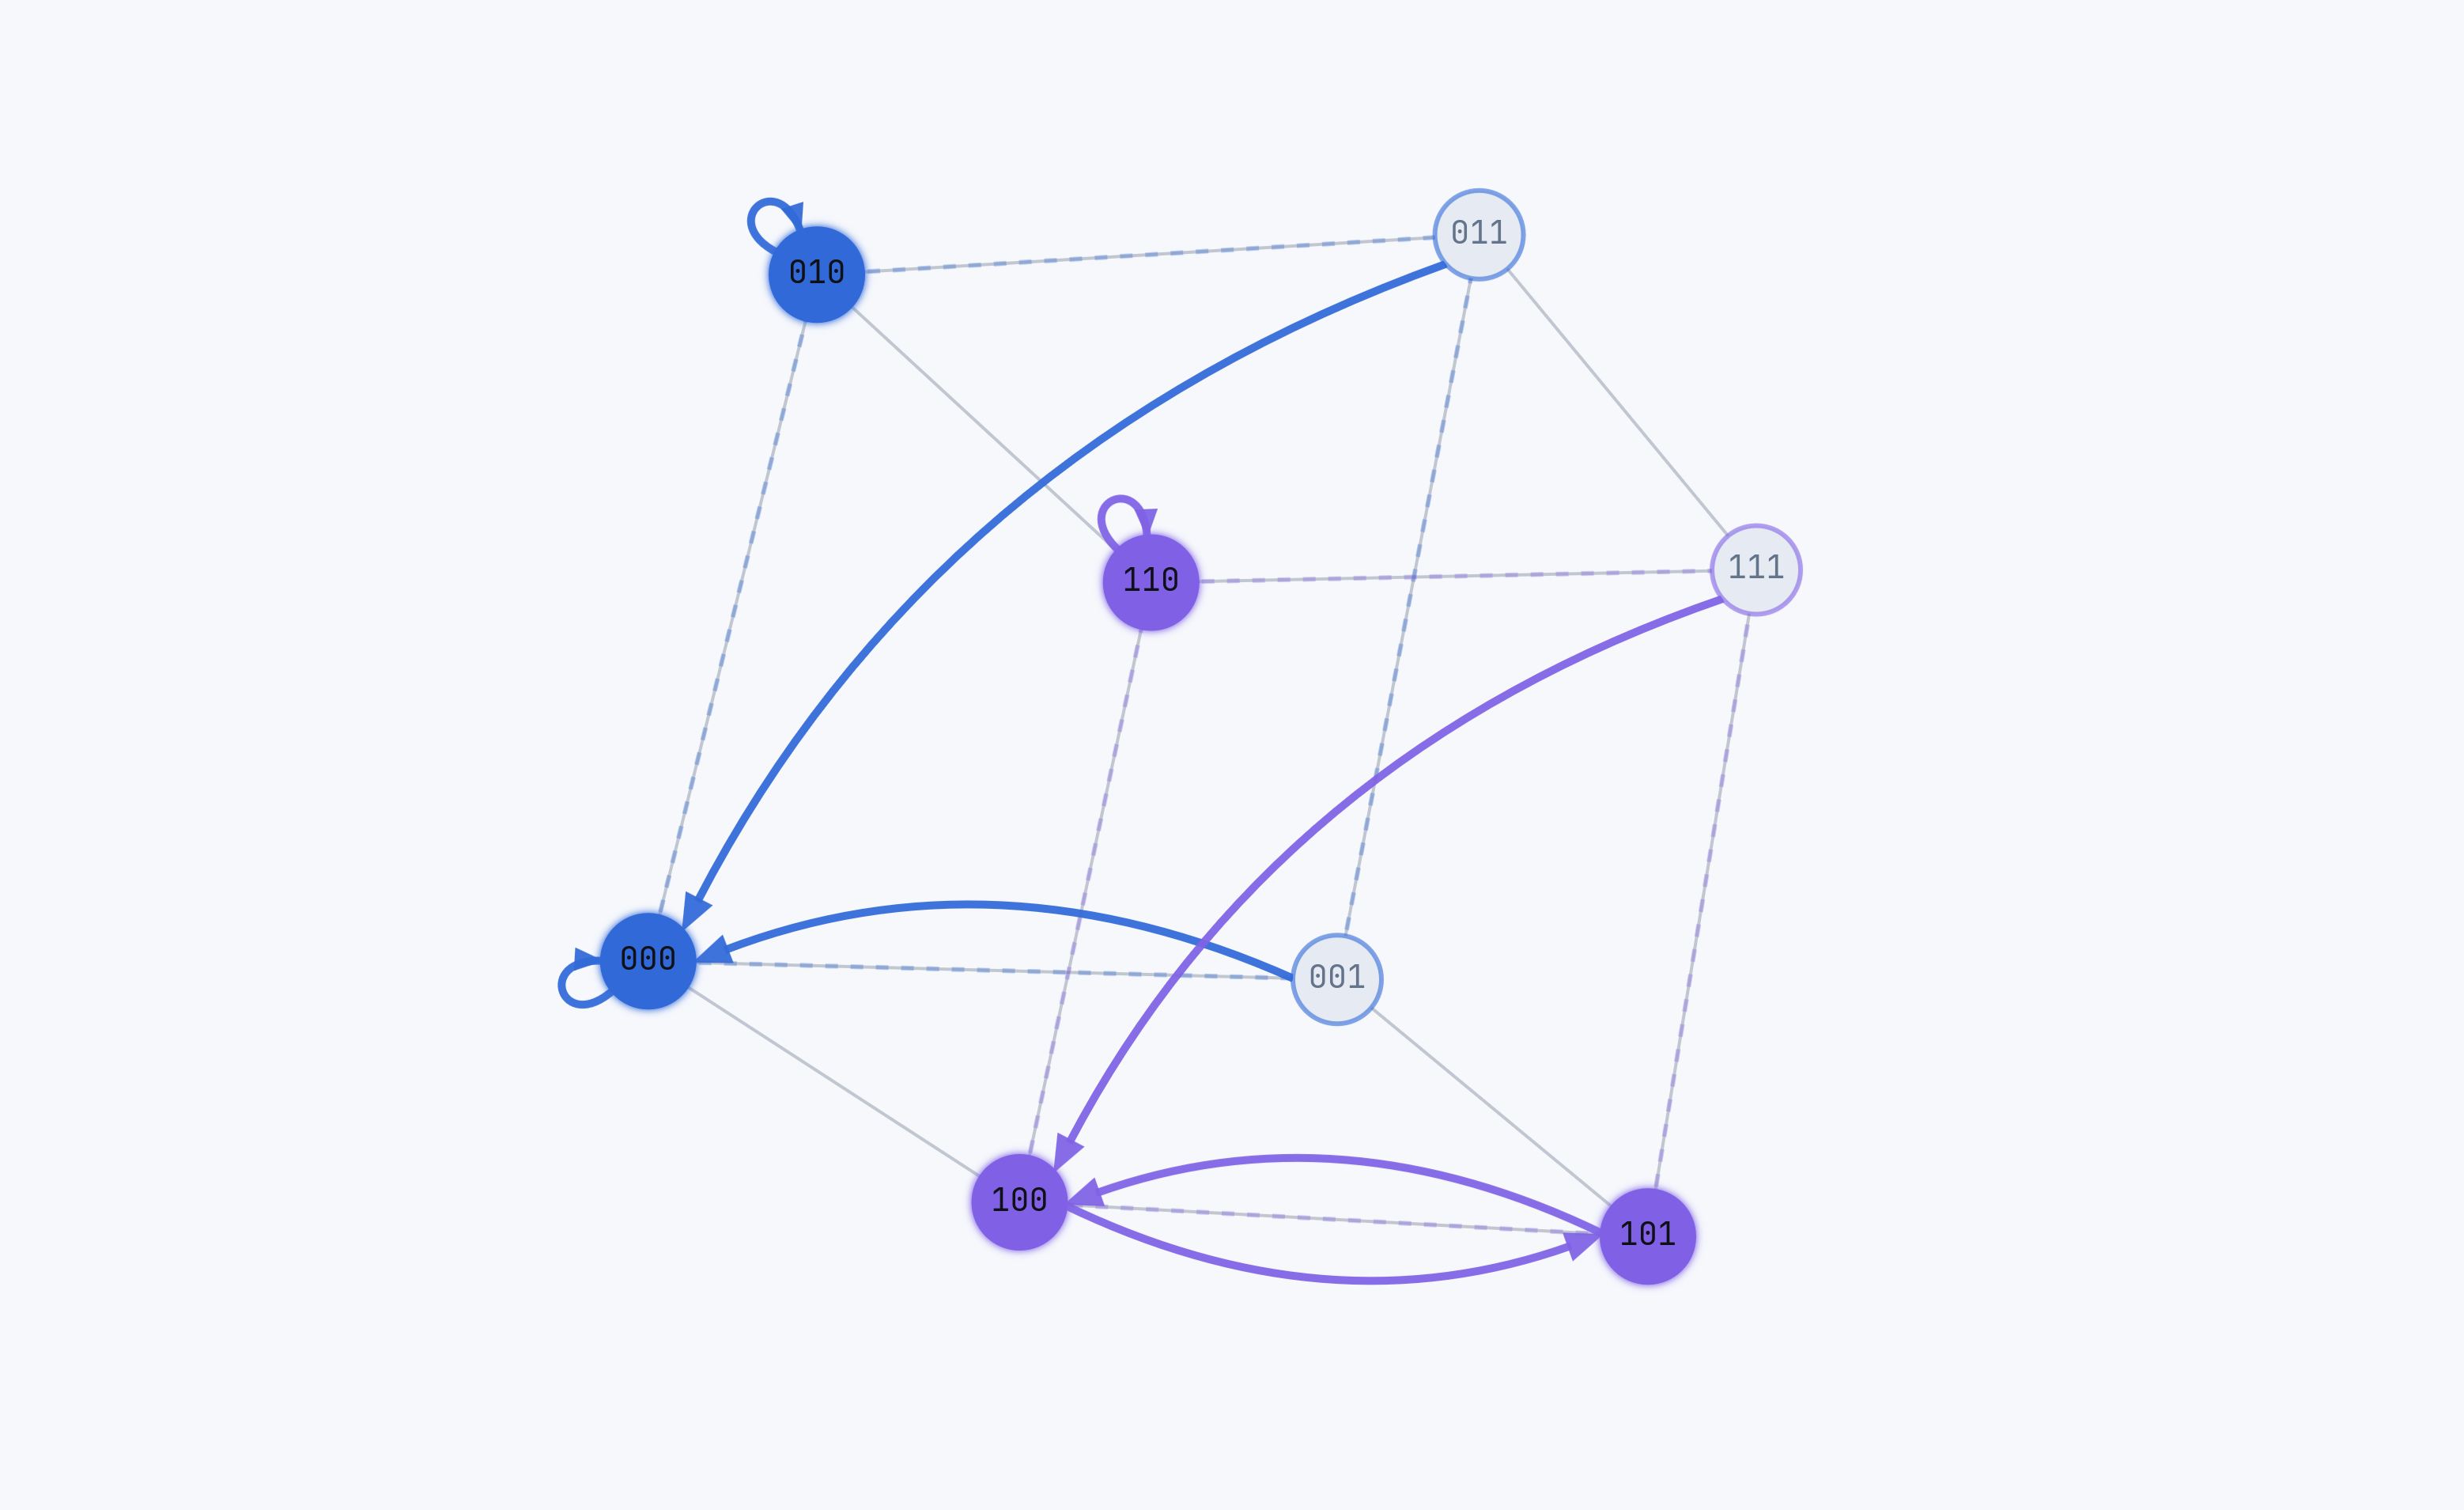
\includegraphics[width=\linewidth]{figures/3d__0_2_0_0__PTBN_undercontrol_taggedtree_sbn71_hypercube.png}
        \caption{Sa dynamique, coloriée par la décomposition.}
    \end{subfigure}
    \caption{Une dynamique décomposable en TBN mais pas en SBN. Le nœud 3 est un nœud de contrôle, mais sur la face $x_3 = 1$ l'état 100 va vers 101, ce qu'aucun SBN ne fait.}
    \label{fig:ptbn-3d}
\end{figure}

Nous avons aussi restreint le domaine des poids eux-mêmes, avec les PSBNI (I pour inhibiteurs), qui sont des PSBN dont les arcs entre nœuds distincts sont inhibiteurs ou absents, $w_{i,j} \le 0$ pour $i \neq j$, les boucles restant libres, ce qui revient à imposer à tous les nœuds la condition que les nœuds de contrôle vérifient déjà sur leurs arcs entrants.
C'est d'ailleurs ce qui les motivait, puisque les propriétés des poids qu'exige la pluripotence devaient être bien plus probables, donc bien plus présentes, dans ce régime, et c'est le cas en dimension 3, où le nœud 3 est un nœud de contrôle (avec des sous-réseaux SBN) pour 36 des 216 dynamiques de ce régime, contre 225 des 32\,768 dynamiques sans restriction.
% src : Quentin, 2026-10-04 (motivation) ; passe unifiée ae10d77 (fiches C1 et P3 : 225 dynamiques
% ⟨0,2,0,0⟩ en PSBN_undercontrol, 36 sur 216 en PSBNI_undercontrol, toutes les 216 sur le vecteur trivial)
% src : PTBNI_undercontrol.lp (domaine -Wb..0 pour I != J) ; Quentin, conv a5891d3a 2026-06-12
% (« pluripotent SBN inhibiteurs pour lesquels les arcs sortant des noeuds ne peuvent être que négatifs »)

% Emplacement de figure (fiche P3) : fiches/3d_P3_PSBNI_undercontrol.csv (n° 235, ⟨0,2,0,0⟩,
% poids 1->1 : +1, 3->1 : -1, 3->3 : +1).
% Fichiers attendus : figures/3d_P3_PSBNI_undercontrol_{reseau,hypercube}.png
\begin{figure}[H]
    \centering
    \begin{subfigure}{0.48\linewidth}
        \centering
        \fbox{\parbox[c][4cm][c]{0.9\linewidth}{\centering Capture à faire (fiche P3)}}
        \caption{La structure.}
    \end{subfigure}
    \hfill
    \begin{subfigure}{0.48\linewidth}
        \centering
        \fbox{\parbox[c][4cm][c]{0.9\linewidth}{\centering Capture à faire (fiche P3)}}
        \caption{Sa dynamique, coloriée par la décomposition.}
    \end{subfigure}
    \caption{Un PSBNI, dont le seul arc entre nœuds distincts, de 3 vers 1, est inhibiteur, et dont le nœud 3 est un nœud de contrôle.}
    \label{fig:psbni-3d}
\end{figure}

Une décomposition peut aussi n'être que partielle, quand des sous-cubes de l'hypercube sont invariants sans que le reste de l'hypercube se laisse découper, comme dans la \Cref{fig:partielle-3d}, où l'arête $\{000, 001\}$ et la face $x_3 = 1$ sont invariantes alors que les états 010 et 011 n'appartiennent à aucune des deux.
C'est une forme de pluripotence que nous n'avons pas explorée (aucun de nos programmes n'énumère ces décompositions partielles), alors qu'elle concerne la plupart des dynamiques, puisqu'en dimension 3, 25\,697 des 29\,791 dynamiques qui n'admettent aucune décomposition, même en TBN, ont pourtant un sous-cube invariant de dimension au moins 1.
% src : passe unifiée ae10d77, fiche P4 (sous-cubes de dimension 1 à n - 1, points fixes exclus) ;
% 29 791 = 32 768 - 2 977 ; présentation de fin de stage, diapo 6 (« non fait »)

% Emplacement de figure (fiche P4) : fiches/3d_P4_PSBN_undercontrol_taggedtree.csv (n° 13 392,
% ⟨1,0,0,0⟩, poids 1->2 : -1, 2->1 : +1, 2->3 : +1, 3->2 : +1, 3->3 : +1). Sous-cubes invariants à
% signaler à la main sur la capture : {000, 001} et {100, 101, 110, 111}.
% Fichiers attendus : figures/3d_P4_PSBN_undercontrol_taggedtree_{reseau,hypercube}.png
\begin{figure}[H]
    \centering
    \begin{subfigure}{0.48\linewidth}
        \centering
        \fbox{\parbox[c][4cm][c]{0.9\linewidth}{\centering Capture à faire (fiche P4)}}
        \caption{La structure.}
    \end{subfigure}
    \hfill
    \begin{subfigure}{0.48\linewidth}
        \centering
        \fbox{\parbox[c][4cm][c]{0.9\linewidth}{\centering Capture à faire (fiche P4)}}
        \caption{Sa dynamique et ses deux sous-cubes invariants.}
    \end{subfigure}
    \caption{Une dynamique sans décomposition complète, dont l'arête $\{000, 001\}$ et la face $x_3 = 1$ sont pourtant invariantes.}
    \label{fig:partielle-3d}
\end{figure}

Enfin, les sous-dynamiques peuvent être décrites par plusieurs coordonnées plutôt que par un seul bit de contrôle.
Dans la dynamique de la \Cref{fig:pcpo-3d}, les nœuds 1 et 2 évoluent seuls, comme un réseau de dimension 2 qui échange leurs valeurs, et le nœud 3 suit selon leur état, gardant sa valeur quand ils sont tous deux éteints et s'éteignant sinon.
J'y vois, par analogie avec le paradigme par lequel j'ai appris le fonctionnement d'un processeur, une partie contrôle (les nœuds 1 et 2) qui pilote une partie opérative (le nœud 3), l'hypercube se partageant en trois supports invariants selon l'attracteur de la partie contrôle, $\{000, 100\}$, $\{011, 111\}$ et $\{001, 010, 101, 110\}$, ce dernier n'étant pas un sous-cube.
Aucun arbre à un seul bit de contrôle ne capte cette organisation, et la dynamique n'a donc que le vecteur trivial.
Par analogie avec l'offuscation d'un code, qui en rend le comportement difficile à lire, nous parlons alors d'offuscation, car les sous-dynamiques existent bien, mais, la partie contrôle comptant plusieurs nœuds, elles ne se distinguent plus selon les faces de l'hypercube.
Cette piste des nœuds contrôlés, à peine esquissée pendant le stage, n'a pas été explorée.
% src : Quentin, 2026-10-04 (sens de « offuscation ») ; Quentin, conv 12941938 2026-10-03 (sous-dynamiques décrites par plusieurs coordonnées ;
% analogie PC/PO) ; passe unifiée ae10d77, fiche P0/P5 (vecteur trivial en PSBN et PTBN, nœuds
% autonomes 1 et 2) ; présentation de fin de stage, diapo 6 (« non fait, mais réfléchi un peu »)

% Emplacement de figure (fiches P0 et P5) : refait la figure sbn6374 du 1er juillet, dont la
% structure ne réalisait pas l'hypercube (bug des poids de treeinsolver, corrigé depuis).
% fiches/3d_P0_PSBN_undercontrol_treeinsolver.csv (n° 84 298, poids 1->2 : +2, 1->3 : -2,
% 2->1 : +2, 2->2 : -1, 2->3 : -1, 3->3 : +1) ; réseau et hypercube depuis la même ligne.
% Fichiers attendus : figures/3d_P0_PSBN_undercontrol_treeinsolver_{reseau,hypercube}.png
\begin{figure}[H]
    \centering
    \begin{subfigure}{0.48\linewidth}
        \centering
        \fbox{\parbox[c][4cm][c]{0.9\linewidth}{\centering Capture à faire (fiches P0 et P5)}}
        \caption{La structure, dont les nœuds 1 et 2 forment la partie contrôle et le nœud 3 la partie opérative.}
    \end{subfigure}
    \hfill
    \begin{subfigure}{0.48\linewidth}
        \centering
        \fbox{\parbox[c][4cm][c]{0.9\linewidth}{\centering Capture à faire (fiches P0 et P5)}}
        \caption{Sa dynamique, dont les supports invariants suivent l'attracteur de la partie contrôle.}
    \end{subfigure}
    \caption{Un réseau organisé en partie contrôle et partie opérative.}
    \label{fig:pcpo-3d}
\end{figure}

